\chapter{Related Work}

Todays use of the internet is heavily based on content dissemination of all kinds of media like audio and video. TV-Shows, clips and tutorials on Youtube, podcasting for educational purposes like on Coursera need to be distributed around the globe. If it is a popular TV-Show the distribution mainly happens within the first few hours of airing. That often leads to a heavy use of bandwith and the bottleneck being the few servers that host that content and their uplinks. In 2008 alone 500 exabytes were created and today's number is a multiple of that [TODO: reference]. That got possible because computers and computing devices became so cheap that almost anybody can afford them. Limited storage on clouds is given free to all users by many providers. When the internet was invented, the situation was a differnet one. There were only a few computers and few resources like tape storage devices, archives or computing power distributed geographically. A client needed some specific information or resources from a specific destination which was known to the client. The client connected through TCP/IP to the Server and after the connection was established and possibly secured the transfer of the information needed by the Client could start. The problem to solve at that time was clearly resource sharing versus today's content dissemination.\\

TCP/IP is no longer best suited for todays use of the internet. One of the main reasons is that a TCP/IP connection is established between two machines only. Content Dissemination best requires a multipoint to multipoint connection. Another reason is that the Client often does not know where to get some specific information from (and doesn't care) but knows exactly what she wants. Therefore a paradigme shift from host-centric networks started to evolve towards content-centric networks.

\section{Named Data Network / Content Centric Networks}

Named Data Network (NDN) is implemented using the Content Centric Networking (CCN) paradigme. In CCN the content is made directly addressable and routable by name. An Interest (request by a client) is sent out and routed according to it's name until it reaches some endpoint that is able to respond with Content Objects to that Interest. Some of the main goals of CCN is better utilization of the bandwith by increasing throughput and decreasing network traffic, better security, availability, flexibility and scalability of the networks. Better utilization of the bandwith can be achieved by multicasting the same content to several endpoints and not re-unicasting the same content over and over again through the same channels near the content source. Also content caching in intermediate nodes reduces the strain on bandwith and increases overall efficiency. Better security is achieved by hashing and signing the content itself instead the point-to-point connection between two hosts. Encrypting the data leads to more privacy within the internet and can substitute many current access policy patterns used by servers and webpages. Better Availability and flexibility are intrinsically given by content caching. Better scalability is achieved by not needing pre-planned structures like CDN's and P2P networks. Data is not only kept at the content producer but everywhere along the route if necessary.

\begin{figure}[h]
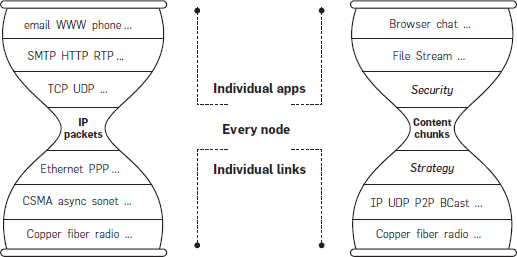
\includegraphics[scale=0.6]{chapter-2/NetworkStack}
\centering
\end{figure}

In Figure 1 the IP and CCN protocol stacks are compared to each other. Both protcol stacks are built in a modular fashion that makes the architecture very flexibl and scalable. The thin waste of the TCP/IP protocol stack consists of IP packages that have a source address and a destination address. This Network Layer is kept very simple and it makes only very weak demands on layer 2. These weak demands on the lower layer make much of the attractivness of IP. This thin waist in TCP/IP protocol stack (\emph{where}) is replaced in CCN with a content layer (\emph{what}) that describes what the package is and has even fewer demands on the lower layer, keeping much of the advantages from IP. Lower layers of the CCN protocol stack are responsible for the routing, encoding and decoding of the information while the higher layers consist of security and the interpretation of the information. Because of the modularity CCN can be implemented on top of IP.

Two big differences of TCP/IP and CNN are the strategy layer and the security layer. The strategy layer is responsible for all dynamic routing decisions based on the name and the strategy. The strategy can be a different one for different namespaces. E.g. an emergency message would be always broadcasted according to it's name. The Security layer differs from the TCP/IP protocal stack since in CCN the content chunks are signed and encrypted instead of securing the connection.

\subsection{CCN/NDN Node Model}

In CCN there are no clients and servers anymore but \textbf{Consumers} and \textbf{Producers}. Consumers request some information by sending out an \textbf{Interest}. This interest packet consists of a content name, some selectors and a nonce. The interest is being forwarded according to the node's strategy until it reaches a node that can satisfy the interest. If a node can satisfy the received interest, it will respond with a \textbf{data} package consisting of the same content name as the interest, a signature, signed info and the data. The data will be sent back towards the consumer. The node having the requested information is called producer (it generates the data) (TODO:is an intermidiate node that does NOT generate it but supports it also a producer???).

\begin{figure}[h]
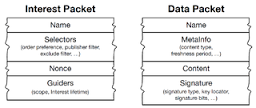
\includegraphics[scale=1]{chapter-2/InterestAndData}
\centering
\end{figure}

The most important data structures for routing the interest to the producer and the data back to the consumer are called the pending interest table (PIT), the forwarding information base (FIB), and the content store (CS).

\subsubsection{PIT}

The Pending Interest Table (PIT) keeps track of all the interests that have been forwarded towards potential content sources. It also keeps track of all incoming and outgoing faces of the specific interests (multiple in-faces and out-faces reflect the multipoint to multipoint characteristics of CCN). When an interest reaches a content source or a producer Data is send back. It follows the breadcrumbs left in the PIT to find it's way back to the consumer. The PIT entries are deleted shortly after the requested Data has been sent downstream.

(TODO: correct place for this or use rather in ndnSIM chapter?) The PIT data structure consists of a PIT entry table that are uniquely identified by the content name of the interest. Further a PIT entry aggregates in-records and out-records. The in-records hold information about the incoming face, nonce, renew date and possibly more information. The out-records hold information about the outgoing face, nonce, renew date and possibly more information.

\subsubsection{CS} 

The Content Store (CS) is located within the intermediate nodes. It is a cache of data packages that have passed this node and have been saved for later use. That is a critical advantage over TCP/IP where data packages are meant only for point to point delivery and cannot be used by other consumers. It depends on the implementation of the CS to decide which packages (solicited and unsolicited) should be saved to the cache and how they should be replaced if the cache is full. Current implementation focus mainly on LRU and LFU replacement strategies. The CS needs to be searched before the interest is handed off to the forwarding strategy.

\subsubsection{FIB}

The Forwarding Information Base (FIB) is used by the strategy to forward Interests upstream towards potential producers or intermediate nodes, that have cached the requested data. Every Interest that needs to be forwarded will be matched against the FIB entries. If an entry is found (longest prefix match) then the interest will be send upstream to the outgoing faces. If there is no match the interest can be broadcast or dropped according to the implementation of the strategy.

(TODO: correct place for this or use rather in ndnSIM chapter?) The FIB data structure consists of a FIB entry table that are uniquely identified by the content name of the interest. These entries aggregate next hops that have an outgoing face and a cost associated with that face.

\subsection{Forwarding of an Interest}

Interests are forwarded based on the content name and the implemented strategy on all intermediate nodes. The above discussed tables are used for deciding if and how to further process the interest. The strategy is only responsible for forwarding the interests towards content sources or producers. The Data coming back follows the path of the interest back to the consumer.

\begin{figure}[h]
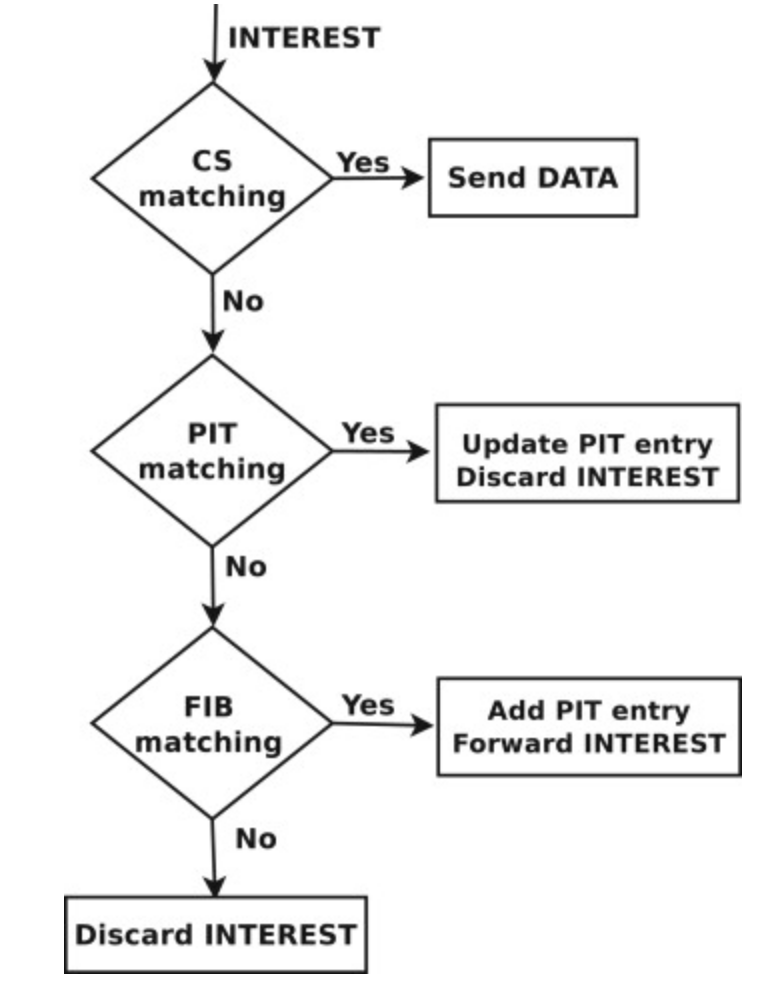
\includegraphics[scale=0.4]{chapter-2/SimpleInterestForwarding}
\centering
\end{figure}

When an interest arrives at some intermediate node the first thing to do is to check if there is already some data in the content store (CS). If the interest can be satisfied by some cached data the data is send downstream towards the consumer and the interest is dropped (not further processed). If the CS has no data with the same content name as in the interest, the PIT entries are checked. If a PIT entry already exists for the interest the node has already requested the data and is awaiting it. The incoming face(s) are added to the existing PIT entry and the interest is dropped. If a PIT entry does not exist yet and no cached data can satisfy the interest, the node needs to forward the interest upstream towards a potential content source. The strategy checks the FIB entries for a longest prefix match. If an entry is found a new PIT entry has to be created with the content name of the interest, it's incoming face and outgoing face (from the FIB). The interest is then forwarded according to the FIB and the strategy.
\\
Sending Data downstream to the original requester is straightforward since no special routing is required. The Data follows the path of the interest left within the PIT entries (in-face(s) of the interest at that node). 

\subsection{Transport and Routing}

As mentioned above the "content chunks" layer in the CCN protocol stack makes even weaker demands on the lower layers then the IP layer makes on layer 2. It operates on unreliable, best-effort packet delivery services in potentially highly dynamic and mobile environments. Interests and Data packages are expected to get lost and/or corrupted. In CNN the strategy layer of the intermediate nodes is responsible to resend the interest if within the timeout no data has been received. The strategy layer knows which outgoing faces were used and what the timeout was, therefore able to adjust the parameters for a retransmission. The same is true for the strategy layer of the consumer. If it does not receive any data back within a given timeframe, it too, will resend (possibly rebroadcast) the interest.
\\
Flow control can be managed by the consumer in terms of how many interests can be sent out before having received the first data packages back. It is also managed on a hop-by-hop basis. Each intermediate node decides when to retransmit an interest due to loss or corrupted data coming back. The buffer for the interests is the PIT whereas the buffer for the data passing downstream to the consumers is the CS. There is no need for special congestion control techniques.

\subsection{Sequencing}

One of the big advantages in CCN over the host-to-host based TCP/IP approach is that the data in transition can be used many times by many different consumers requesting the same data possibly far away from the original producer. That leads to the problem of uniquely identifying the data in a self explanatory way. Consumers must be able to deterministically construct a name for the data without having previously seen it. Hierarchical names that reflect the content and the organizational structure of their origin are very well suited to solve that problem. Since the naming is absolutely irrelevant for the network, applications can choose a naming that fits their need best. For example, to get the segment 34 of a video version 2 by group A of the University of Bern the name could be:

/unibe.ch/group/A/videos/introduction.mpg/_v2/_s32

This name can be aggregated with more components if needed by the application or network. It only needs to adhere to previously specified rules.


\subsection{Content-Based Security}

CCN digitally signes and encrypts the content itself and not the connection over which it travels. TCP/IP needs to secure the connections which in turn must link the content to the server infrastructure. To trust a content the user must fetch it from it's original source making it very difficult to cache popular content and make it available to other users.

\section{VANETS}
